\section{Gaussian Mixture Model (GMM)}
\label{sec:gmm}
% univariate Gaussian
In its univariate form, a Gaussian or normal distribution is defined by
\begin{equation}
	\gaussian{x\vert\mu,\sigma}=\frac{1}{(2\pi\sigma^2)^{1/2}}\exp\left\{-\frac{1}{2\sigma^2}(x-\mu)^2\right\},
\end{equation}
where $\mu$ is called its \textit{mean} and $\sigma^2$ is called its \textit{variance}.
%This distribuion satisfies the requirements $\int_{-\infty}^{\infty}\gaussian{x\vert\mu,\sigma^2}\text{d}x=1$ and $\gaussian{x\vert\mu,\sigma^2}>0\ \forall\ x\in\mathbb{R}$, which qualifies the Gaussian distribution as a probability distribution.
The multivariate Gaussian distribution for an input vector $\bm x\in\mathbb{R}^D$ is defined by
\begin{equation}
	\gaussian{\bm x\vert\bm\mu,\bm\Sigma}=\frac{1}{(2\pi)^{D/2}}\frac{1}{\bm\Sigma^{1/2}}\exp\left\{-\frac{1}{2}(\bm x-\bm\mu)^{\text{T}} \bm\Sigma^{-1}(\bm x-\bm\mu)\right\}.
\end{equation}



% Complexity of multivariate Gaussians
Compared to the univariate form with only two free parameters, this \gls{pdf} is completely defined by its covariance matrix $\bm\Sigma\in\mathbb{R}^{D\times D}$ and its mean vector $\bm\mu\in\mathbb{R}^D$. As the covariance matrix is symmetric, is has $D(D+1)/2$ independent parameters (assuming it is positive definite). Adding the $D$ independent parameters of $\bm\mu$ results in $D(D+3)/2$ independent parameters that define a multivariate Gaussian distribution. 

The complex variant of the Gaussian distribution is defined by
\begin{equation}
    \mathcal{N}^c(\bm z,\Gamma)=\frac{1}{\pi^N\cdot\text{det}\ \Gamma}\exp\{ -\bm z^*\Gamma^{-1}\bm z \},
    \label{eq:complexGaussian}
\end{equation}
where $\bm z\in\mathbb{C}^N$, $\Gamma$ is the complex covariance matrix, $\text{det}\ \Gamma$ is the determinant of $\Gamma$, $\bm z^*$ denotes the complex conjugate of $\bm z$ and $\Gamma^{-1}$ the inverse of $\Gamma$. 

% not really needed
%As shown in \cite{Gallager2008}, for the density of $m$ independent circular-symmetric Gaussian random variables, this can be written using the eigenvalues $\lambda_j$ and eigenfunction $\bm q_j$ of the covariance matrix
%\begin{equation}
%\label{eg:complexGaussianDef}
%    \mathcal{N}^c(\bm z,\lambda_j)=\prod_{j=1}^n\frac{1}{\pi\lambda_j}\exp(-|z,q_j|^2\lambda_j^{-1}).
%\end{equation}
%This formulation will be used when modelling the \gls{prp} using a \gls{gmm}.\\

% from single gaussian to mixture model
Despite possessing these many degrees of freedom, the Gaussian distribution is limited in a sense, that it has only one maximum (\textit{unimodality}) and therefore cannot adequately model multimodally distributed data. To overcome this limitation, multiple Gaussians can be combined into what is called a \acrlong{gmm}

% the GMM
\begin{equation}
	p(\bm x)=\sum^J_{j=1}\psi_j\cdot\gaussian{\bm x\vert\bm\mu_j,\bm\Sigma_j},
\end{equation}

where $\psi_j$ is the weighting factor or \textit{mixing coefficient} of each Gaussian component $\gaussian{\bm x\vert\bm\mu_j,\bm\Sigma_j}$ of the \gls{gmm} with $0\leq\psi_j\leq 1$ and $\sum_{j=1}^J \psi_j=1$. In addition to $\bm\mu=[\bm\mu_1,\dots,\bm\mu_J]$ and $\bm\Sigma=[\bm\Sigma_1,\dots,\bm\Sigma_J]$, each a concatenation of the parameters of the multivariate Gaussian for each component $j$, the \gls{gmm} has a third parameter $\bm\psi=[\psi_1,\dots,\psi_J]$. An example of a Gaussian mixture with three components is shown in \autoref{fig:gaussianmixture}. The parameters of a \gls{gmm} can be calculated under the Maximum-Likelihood criterion as follows:

\begin{equation}
	\text{ln}\ p(\bm X\vert\bm\psi,\bm\mu,\bm\Sigma)=\sum_{n=1}^N \text{ln}\left\{\sum_{j=1}^J \psi_k\cdot\gaussian{\bm x_n\vert\bm\mu_j,\bm\Sigma_j} \right\},
\end{equation}

with $\bm X=\{\bm x_1,\dots,\bm x_N\}$. As a result of the presence of the sum inside the logarithm, the \gls{ml} solution for these parameters does not have a closed-form solution \cite[p.~113]{Bishop2006}. One way to solve these type of \gls{ml} problems is the \gls{em} algorithm presented in the following section. By introducing a latent random variable that models the missing information, the \gls{em} algorithm makes the \gls{ml} problem tractable.

\begin{figure}[!hbt]
    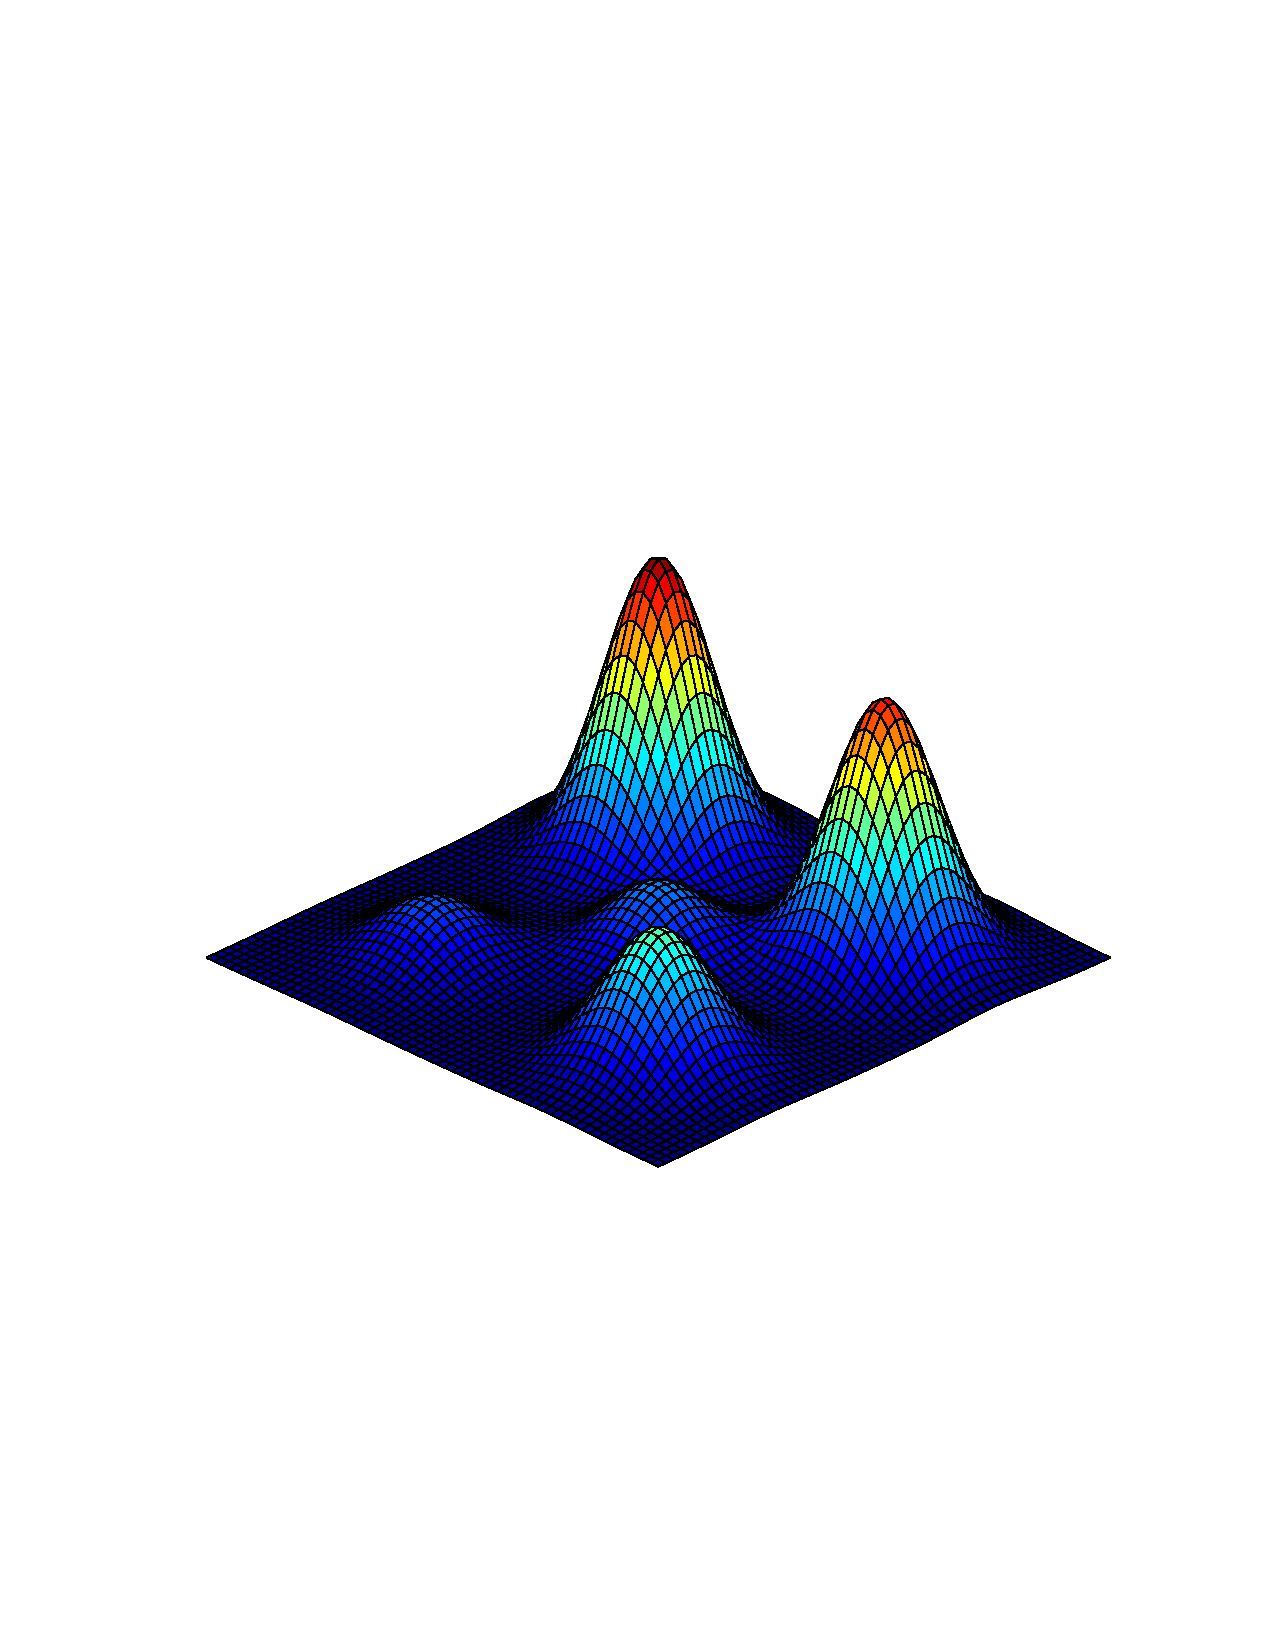
\includegraphics[width=6cm]{plots/gmm/gaussian}
    \caption[Example of a Gaussian Mixture]{A Multivariate Gaussian Mixture with $j=5$ Weighted Components.}
    \label{fig:gaussianmixture}
\end{figure}

